\chapter{Matching su Grafi Bipartiti}

Ora che abbiamo visto e sviluppato degli algoritmi potenti ed efficaci
per il problema del Flusso Massimo, è ora di vedere le applicazioni di
quest'ultimi per alcuni problemi noti. Durante l'introduzione del
Problema del Flusso Massimo, abbiamo introdotto il
\textbf{\emph{Bipartite Matching Problem}}, inizieremo quindi con la
risoluzione di quest'ultimo e, successivamente, affronteremo il
\textbf{\emph{Disjoint Paths Problem}}.

\section{Descrizione del problema}

Ricordando che un \emph{grafo bipartito} $G = (V, E)$ è un grafo non
orientato il cui insieme di nodi può essere partizionato come
$V = X \cup Y$, con la proprietà che ogni arco $e \in E$ ha una fine
in $X$ e l'altra in $Y$ (ogni arco connette un nodo in $X$ e uno
in $Y$).\\ Un \textbf{matching} $M$ in $G$ è un sottoinsieme di
archi $M \subseteq E$ tale che ogni nodo appare in al massimo un arco
in $M$. Il \textbf{\emph{Bipartite Matching Problem}} consiste nel
trovare il matching in $G$ più grande possibile (matching di
\textbf{cardinalità massima}).

\section{Designing the Algorithm}

Il grafo in questione è indiretto, mentre le reti di flusso sono
dirette, tuttavia non è difficile applicare un algoritmo per il Problema
del Massimo Flusso per trovare un matching massimo, vediamo come:\\

Dato un grafo $G$ come istanza per il Bipartite Matching Problem, si
costruisce una rete di flusso $G'$ come mostrato nella Figura qui di
seguito:\\

\begin{figure}[H]
	\centering
	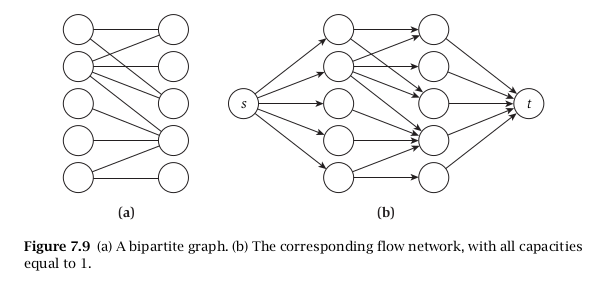
\includegraphics[width = 12cm]{capitoli/network_flow/imgs/bipartite1.png}
	\caption{Corrispondenza tra grafo bipartito e flow network}
\end{figure}

Come si ottiene $G'$ ?
\begin{itemize}
	\item Per prima cosa si direzionano tutti gli archi di $G$ che vanno da $X$ a $Y$
	\item Si aggiunge poi un nodo $s$, e un arco $(s, x)$ da $s$ ad ogni nodo in $X$
	\item Si aggiunge un altro nodo $t$, e un arco $(y, t)$ da ogni nodo in $Y$ verso $t$
	\item Infine, si da una capacità di 1 ad ogni arco in $G'$
\end{itemize}

Si può ora calcolare il massimo flow $s-t$ nella rete $G'$.\\

Vedremo ora come:
\begin{itemize}
	\item \textbf{Il valore del massimo flusso di questa rete ($G'$) in
		      realtà è uguale alla dimensione del massimo matching in $G$.}
	\item Inoltre vederemo come ricostruire il matching utilizzando il flusso della rete.
\end{itemize}

\paragraph{Dimostrazione del primo punto}

$\leftarrow$\\
Si supponga l'esistenza di un matching in $G$ composto da $k$
archi $(x_{i_1}, y_{i_1}), ..., (x_{i_k}, y_{i_k})$ Si consideri
allora un flusso $f$ che trasporta un'unità su ogni path dalla
struttura $s, x_{i_j}, y_{i_j}, t$ con $f(e) = 1$ per ogni arco per
ognuno dei cammini. Si può verificare facilmente che le condizioni di
capacità e la conservazione sono verificate e che $f$ è un flusso
$s-t$ di valore $k$\\

$\rightarrow$\\
Dall'altro lato, si supponga l'esistenza di un flusso $f'$ in
$G'$ di valore $k$. Dal teorema dell'integralità del massimo flusso
\protect\hyperlink{def-714}{7.14}, sappiamo che esiste un flusso $f$
di valore intero $k$; e siccome tutte le capacità sono $1$, questo
significa che $f(e)$ è uguale a 0 o 1 per ogni arco $e$. Si
consideri ora un insieme $M'$ di archi dalla forma $(x, y)$ sui
quali il flusso ha valore 1.\\

Ecco 3 semplici fatti sull'insieme $M'$:
\begin{itemize}
	\item $M'$ contiene $k$ archi
	\item Ogni nodo in $X$ è la coda di al massimo un arco in $M'$
	\item Ogni nodo in $Y$ è la testa di al massimo un arco in $M'$
\end{itemize}

Combinando questi fatti, vediamo che se consideriamo $M'$ come un
insieme di archi nel grafo bipartito originale G, otteniamo un matching
di dimensione $k$. In sintesi, abbiamo dimostrato il seguente fatto.

\begin{myblockquote}
	La dimensione del massimo matching in $G$ è uguale al valore del
	massimo flusso in $G'$ ; e gli archi in un tale matching in G sono gli
	archi che portano il flusso da $X$ a $Y$ in $G'$.
\end{myblockquote}

\subsection{Costo}

Sia $n = |X| = |Y|$, e sia $m$ il numero di archi di $G$.
Assumiamo che ci sia un arco entrante in ogni nodo, e quindi
$m \ge n/2$. Il tempo per computare il massimo matching è dominato dal
tempo per computare un maximum flow a valore intero in $G'$, quindi
convertire quest'ultimo ad un matching in $G$ è facile. Per questo
problema di flusso, abbiamo che
$C = \sum_{e \text{ out of } s}c_e = |X| = n$, con $s$ come arco di
capacità 1 per ogni nodo di $X$. Quindi, utilizzando $O(mC)$ come
bound (limite), abbiamo il seguente corollario:
\begin{myblockquote}
	L'algoritmo di \texttt{Ford-Fulkerson} può essere utilizzato per trovare
	un matching massimo in un grafo bipartito in tempo $O(mn)$.
\end{myblockquote}


\section{Perfect Matching}

Dato un grafo non diretto $G=(V,E)$, $M \subseteq E$ è un
\textbf{matching perfetto} se ogni vertice $v \in V$ compare in $M$
esattamente una volta.
\begin{itemize}
	\item Dobbiamo avere \textbar X\textbar{} = \textbar Y\textbar{}
\end{itemize}

\textbf{Notazione}: Sia $S$ un sottoinsieme dei nodi, e sia $N(S)$
l'insieme dei nodi adiacenti ai nodi in $S$

\begin{myblockquote}
	\textbf{Se un grafo bipartito $G = (V, E)$, con i due lati $X$ e
		$Y$, ha un perfect matching, allora per ogni $S \subseteq X$ si deve
		avere $|N(S)| \ge |S|$.}
\end{myblockquote}

\textbf{Dimostrazione} Ogni nodo in $S$ deve essere matchato a un
differente nodo in $N(S)$\\

\begin{figure}[H]
	\centering
	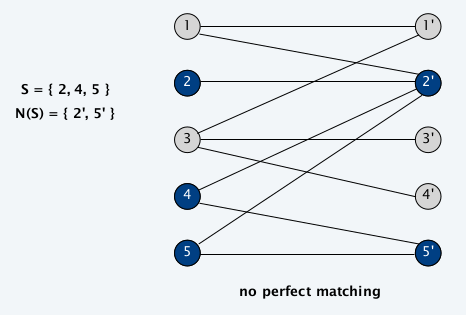
\includegraphics[width = 10 cm]{capitoli/network_flow/imgs/bipartite2.png}
	\caption{esempio di assenza di matching perfetto}
\end{figure}

Con l'affermazione precedente possiamo anche constatare quando un grafo
non ha un matching perfetto:
\begin{itemize}
	\item un insieme $S \subseteq X$ tale per cui $|N(S)| < |S|$
\end{itemize}

Da qui ne deriva un teorema chiamato \textbf{Hall's Theorem}, la cui
dimostrazione fornisce anche un modo per trovare il sottoinsieme $S$
in tempo polinomiale.

\subsection{Hall's Theorem}

Sia $G=(V, E)$ un grafo bipartito con i due lati $X$ e $Y$, tali
per cui $|X| = |Y|$. Allora G ha un perfect matching oppure c'è un
sottoinsieme $S \subseteq X$ tale per cui $|N(S)| < |S|$. Un
matching perfetto o un appropriato sottoinsieme $S$ può essere trovato
in tempo $O(mn)$.\\

\textbf{Dimostrazione:}\\
$\Rightarrow:$\\
Ogni nodo in $S$ deve essere
collegato ad un nodo al di fuori di $N(S)$ (al di fuori di $S$). (Si
noti come questa è la stessa dimostrazione della precedente
affermazione.)\\

$\Leftarrow:$\\
Suppongo che G \textbf{non} abbia perfect matching.
\begin{itemize}
	\item Lo si formuli come un max-flow problem e sia $(A,B)$ un min-cut di $G'$.
	\item Dal max-flow min-cut theorem $cap(A,B) < |X|$.
	\item Definisco $X_A = X \cap A$, $X_B = X \cap B$, $Y_A = Y \cap A$
	\item $cap(A,B) = |X_B| + |Y_A| \implies |Y_A| < |X_A|$
	\item min-cut non può usare archi con capacità infinita $\implies N(X_A) \subseteq Y_A$
	\item $|N(X_A)| \le |Y_A| < |X_A|$ - scelgo $S = X_A$. \textbf{Il che è assurdo}.
\end{itemize}

\begin{figure}[H]
	\centering
	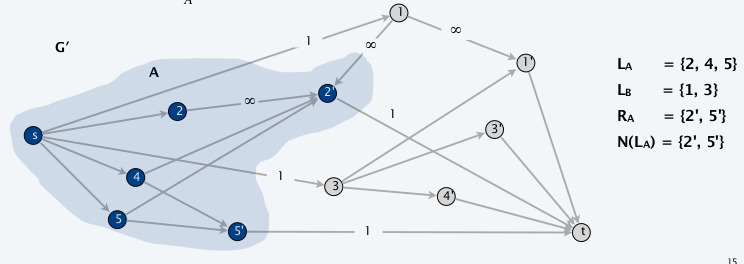
\includegraphics[width = 12 cm]{capitoli/network_flow/imgs/bipartite3.png}
\end{figure}

Si noti che $X$ corrisponde a $L$ e $Y$ a $R$ nella figura.

\section{Disjoint Paths}

\subsection{Descrizione del problema}

Due path sono \textbf{edge-disjoint} se non hanno archi in comune.\\

\textbf{Edge-Disjoint Paths Problem:} dato un grafo $G$ e due nodi
$s$ e $t$, trovare il massimo numero di \textbf{edge-disjoint path}
da $s$ a $t$.


\subsection{Max-Flow Formulation}

Assegno capacità 1 ad ogni arco\\

\textbf{Teorema}

Il massimo numero di edge-disjoint $s-t$ paths = valore del max-flow\\

\textbf{Dimostrazione:} $\le:$
\begin{itemize}
	\item Suppongo che ci siano $k$ edge-disjoint paths da s a t.
	\item Pongo $f(e)=1$ per tutti gli archi che compaiono in questi path, altrimenti pongo $f(e)=0$.
	\item Dato che non ci sono archi in comune, $f$ è un flow di valore $k$.
\end{itemize}

$\ge:$
\begin{itemize}
	\item Suppongo che il max-flow abbia valore $k$.
	\item Per l'integrality theorem esiste un flow $0-1$ di valore $k$.
	\item Considero gli archi $(s, u)$ con $f(s, u) = 1$.
	      \begin{itemize}
		      \item Per la conservazione del flusso esiste un arco $(u,v)$ con $f(u, v) = 1$.
		      \item Continuo scegliendo sempre nuovi archi fino a raggiungere $t$.
	      \end{itemize}
	\item Produco $k$ edge-disjoint paths.
\end{itemize}

\section{Network Connectivity}

\subsection{Descrizione del problema}

Un set di archi $F \subseteq E$ \textbf{disconnette} $t$ da $s$ se
ogni path da $s-t$ passa per almeno un arco di $F$.\\

\textbf{Network Connectivity:} Dato un digrafo $G = (V,E)$ e due nodi
$s$ e $t$, trovare il minor numero di archi la cui rimozione porta
alla disconnessione di $t$ da $s$.\\

\subsection{Teorema di Menger}

Il numero massimo di edge-disjoint $s-t$ paths = numero minimo di
archi la cui rimozione porta alla disconnessione di $t$ da $s$.\\

\textbf{Dimostrazione:} $\le:$
\begin{itemize}
	\item Suppongo che la rimozione di $F \subseteq E$ disconnetta $t$ da $s$ e $|F| = k$.
	\item Ogni path $s-t$ passa per almeno un arco di $F$.
	\item Quindi il numero di edge-disjoint path è $\le k$
	\item \begin{figure}[H]
		      \centering
		      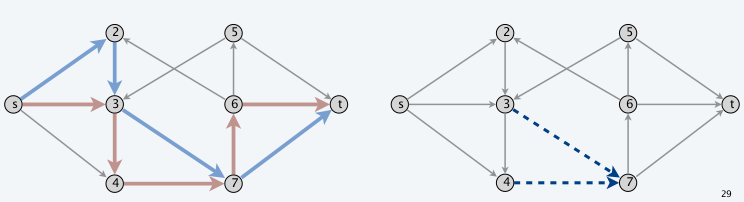
\includegraphics[width = 12cm]{capitoli/network_flow/imgs/bipartite4.png}
	      \end{figure}
\end{itemize}

$\ge :$
\begin{itemize}
	\item Suppongo che il massimo numero di edge-disjoint path sia $k$.
	\item Allora, il Max-flow value è $k$.
	\item Per il max-flow min-cut theorem esiste un cut $(A,B)$ di capacità $k$.
	\item Sia $F$ l'insieme di archi che vanno da $A$ a $B$.
	\item $|F| = k$ e disconnette $t$ da $s$.
	\item  \begin{figure}[H]
		      \centering
		      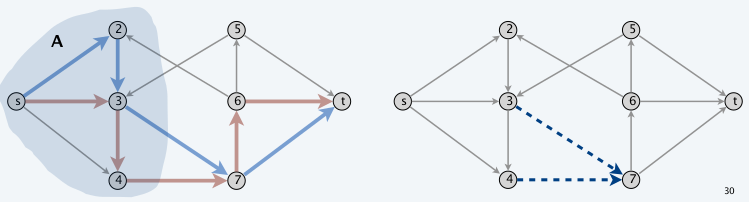
\includegraphics[width = 12cm]{capitoli/network_flow/imgs/bipartite5.png}
	      \end{figure}
\end{itemize}

%\end{document}
